
Grouping messages or aggregating tags introduces dependencies in the verification process, making the system more vulnerable to jamming attacks. By constructing the dependency graph, we model the relationships between messages and tags.

% Next, we define critical metrics: Comparative Efficiency ($CE$), authentication ($\textbf{A}$), latency ($\textbf{L}$), strength number, number of tag-bits per message,\tianwei{should we also have abbreviation for these two metrics here?} and goodput ($G$). These metrics are essential for assessing the robustness and resiliency of MAC overhead-reducing schemes under jamming or insider attacks.\tianwei{some metrics in Table 1 are not mentioned here, does that mean they are not critical? should we add some explanations for why we consider these are essential?}

% \begin{table}[h]
% \centering
% \caption{Summary of Metrics and Acronyms}
% \begin{tabular}{|c|c|}
% \hline


% \multicolumn{2}{|c|}{ \cellcolor[HTML]{D3D3D3} \large \textbf{Vectors} }\\ \hline

% \textbf{Metric} & \textbf{abbrv.} \\ \hline

% Authentication & \textbf{A} \\\hline
% Expected Number of Authentications & $E[\textbf{A}]$ \\ 
% \hline 
% Authenticationd Latency & \textbf{L} \\ \hline

% Tag Usability & \textbf{U} \\ \hline

% Dependency  Matrix & \textbf{X} \\ \hline
% % \multicolumn{2}{c}{}\\
% \hline
% \multicolumn{2}{|c|}{\cellcolor[HTML]{D3D3D3} \large Scalars}\\ \hline
% \textbf{Metric} & \textbf{abbrv.} \\ \hline

% Comparative  Efficiency &$CE$  \\ \hline


% Goodput & $G$ \\ \hline

% Integrity Security & $IS$ \\ \hline

% Strength Number &$SN$\\ \hline
% \end{tabular}
% \label{tab:metrics}
% \end{table}



\subsection*{\textbf{Dependency Graph}}
Assuming the general case of a system with '$m$' messages and '$n$' tags where:
\begin{align}
    \textbf{m} = \{m_1, m_2, \cdots, m_i, \cdots, m_m\}\nonumber\\
    \textbf{t} = \{t_1, t_2,\cdots, t_j,\cdots, t_n\}\nonumber
\end{align}

We define the dependency graph such that \( DG = (\textbf{V}, \textbf{E}) \) is an undirected graph representing the tag-to-message dependencies.  \( DG \) is defined as follows:
\begin{equation}
    \textbf{V}_1 = \{m_i\mid i \in \{1,\cdots,m\}\},\nonumber
\end{equation}
is the set of vertices, where each \( m_i \) represents a message.
\begin{equation}
    \textbf{V}_2 = \{t_j\mid j \in \{1,\cdots,n\}\}, \nonumber
\end{equation}
is the set of vertices, where each \( t_j \) represents a tag, And 
\begin{equation}
    \textbf{V} = \textbf{V}_1 \cup \textbf{V}_2\nonumber.
\end{equation}
\begin{equation}
    \textbf{E} \subseteq\{ (u, v) \mid u \in \textbf{V}_1, v \in \textbf{V}_2\}, \nonumber 
\end{equation}
is the set of undirected edges, where an edge \( \{m_i, t_j\} \in \textbf{E} \) signifies that tag \( t_j \) verifies message \( m_i \).

Each vertex \( v \in \textbf{V} \) can be a message or tag, and each edge \( e \in \textbf{E} \) indicates a tag-to-message assignment. Figure~\ref{fig:proMAC_graph} visualizes the dependency graph for the progressive MAC.
\begin{figure}[!h]
    \centering
    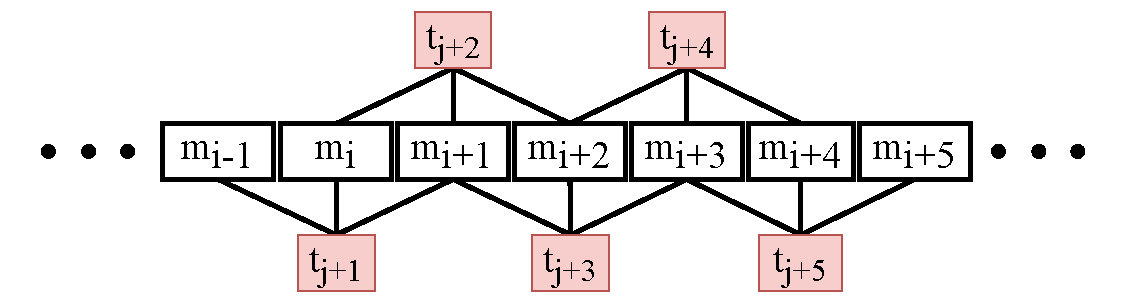
\includegraphics[width = .9\columnwidth]{img/graph/Whip_Graph.pdf}
    \caption{Whips dependency graph with internal state size of 3.}
    \label{fig:proMAC_graph}
\end{figure}

\subsection*{\textbf{Dependency Matrix (X)}}Based on the dependency graph, we define the dependency matrix \( X \), where the rows correspond to messages and the columns correspond to tags. The entries of the matrix are defined as follows:
\begin{equation}
X_{i,j} = 
\begin{cases} 
1 & \text{if message } m_i \text{ is assigned to tag } t_j \\
0 & \text{otherwise}
\end{cases}
\end{equation}

For example, the dependency matrix of the Whips scheme, as shown in Figure~\ref{fig:proMAC_graph}, is as follows:
\setlength{\tabcolsep}{1.9pt}
\renewcommand{\arraystretch}{1.3}
\[
\begin{array}{ccccccccc}
\multirow{12}{*}{\textbf{X} =}& & \textcolor{red!40}{t_1} & \cdots & \textcolor{red!40}{t_{j+1}} & \textcolor{red!40}{t_{j+2}} & \textcolor{red!40}{t_{j+3}}  &  \cdots & \textcolor{red!40}{t_n} \\
\cline{3-3}
\cline{9-9}
&\textcolor{blue!60}{m_1}     & \multicolumn{1}{|c}{1} & \cdots  & 0 & 0 & 0 & \cdots & \multicolumn{1}{c|}{0} \\
&\vdots & \multicolumn{1}{|c}{\vdots} & \ddots & \vdots & \vdots & \vdots & \ddots &  \multicolumn{1}{c|}{\vdots} \\
&\textcolor{blue!60}{m_{i-1}} & \multicolumn{1}{|c}{0} &  \cdots & 1 & 0 & 0 & \cdots & \multicolumn{1}{c|}{0} \\
&\textcolor{blue!60}{m_{i}}   & \multicolumn{1}{|c}{0} &  \cdots & 1 & 1 & 0 & \cdots & \multicolumn{1}{c|}{0} \\
&\textcolor{blue!60}{m_{i+1}} & \multicolumn{1}{|c}{0} &  \cdots & 1 & 1 & 1 & \cdots & \multicolumn{1}{c|}{0} \\
&\textcolor{blue!60}{m_{i+2}} & \multicolumn{1}{|c}{0} &  \cdots & 0 & 1 & 1 & \cdots & \multicolumn{1}{c|}{0} \\
&\textcolor{blue!60}{m_{i+3}} & \multicolumn{1}{|c}{0} &  \cdots & 0 & 0 & 1 & \cdots & \multicolumn{1}{c|}{0} \\
&\vdots & \multicolumn{1}{|c}{\vdots} & \ddots & \vdots & \vdots & \vdots  & \ddots &  \multicolumn{1}{c|}{\vdots} \\
& \textcolor{blue!60}{m_m} & \multicolumn{1}{|c}{0} & \cdots & 0 & 0 & 0 &    \cdots & \multicolumn{1}{c|}{1} \\
\cline{3-3}
\cline{9-9}
\end{array}
\]


% \[
% \begin{array}{ccccccc}
% \multirow{8}{*}{X =}& & \textcolor{red!40}{r_{j+1}} & \textcolor{red!40}{r_{j+2}} & \textcolor{red!40}{c_{j+1}} & \textcolor{red!40}{c_{j+2}}  &  \textcolor{red!40}{c_{j+3}} \\
% \cline{3-3}
% \cline{7-7}
% &\textcolor{blue!60}{m_{i+1}} & \multicolumn{1}{|c}{1} & 0 & 1 & 0 &\multicolumn{1}{c|}{0} \\
% &\textcolor{blue!60}{m_{i+2}} & \multicolumn{1}{|c}{1} & 0 & 0 & 1 &\multicolumn{1}{c|}{0} \\
% &\textcolor{blue!60}{m_{i+3}} & \multicolumn{1}{|c}{1} & 0 & 0 & 0 &\multicolumn{1}{c|}{1} \\
% &\textcolor{blue!60}{m_{i+4}} & \multicolumn{1}{|c}{0} & 1 & 1 & 0 &\multicolumn{1}{c|}{0} \\
% &\textcolor{blue!60}{m_{i+5}} & \multicolumn{1}{|c}{0} & 1 & 0 & 1 &\multicolumn{1}{c|}{0} \\
% &\textcolor{blue!60}{m_{i+6}} & \multicolumn{1}{|c}{0} & 1 & 0 & 0 &\multicolumn{1}{c|}{1} \\

% \cline{3-3}
% \cline{7-7}
% \end{array}
% \]

\subsection*{\textbf{Status Vector}} Let \( \mathbf{M} \) and \( \mathbf{T} \) denotes the status vector, where each entry indicates if the message or tag is correctly received or lost (modified or jammed). \( \mathbf{M} \) is defined as follows:
\[
\mathbf{M} = 
\begin{bmatrix}
M_1 & M_2 & M_3 & \cdots& M_i & \cdots & M_m 
\end{bmatrix}
\]
Where \( M_i = 1 \) if message \( m_i \) is successfully received, and \( M_i = 0 \) otherwise. The tag status vector \( \mathbf{T} \) is defined as follows:
\[
\mathbf{T} = 
\begin{bmatrix}
T_1 & T_2 & T_3 & \cdots & T_j & \cdots & T_n
\end{bmatrix}
\]
Where \( T_j = 1 \) if tag \( t_j \) is successfully received, and \( T_j = 0 \) otherwise. 


% Assuming that tags and messages are sent separately is the most general case, covering all possible implementations. By simply setting the tag status vector to all 1s, we can represent implementations where tags are sent alongside the messages. This is based on the assumption that the tag $t_j$ next to message $m_i$ must at least verify $m_i$. 
% If the packet containing both $m_i$ and $t_j$ is lost, even though in the tag status vector $T_j =1$, the inherent relationship between $m_i$ and $t_j$ means that $M_i = 0$ should effectively result in $T_j = 0$.






\subsection*{\textbf{Tag Usability (U)}}
A tag is usable if the tag and all the dependent messages are correctly received. Let $U_j = 1$ if tag $t_j$ is usable, and $U_j = 0$ otherwise. A usable tag can authenticate all the messages that are dependent on it, whereas an unusable tag can not verify any messages. the $U_j$ in the tag usability vector \( \textbf{U} =  \{U_1, ..., U_n\}\) is given by:
\begin{equation}    
U_j = T_j \cdot \prod_{i \in \{i \mid X_{ij} = 1\}} M_i
\end{equation}

\subsection*{\textbf{Authentication (A)}}
Let $A_i$ denote the number of usable tags verifying message $m_i$. The $A_i$ from the authentication vector $\textbf{A} = \{A_1, ..., A_m\}$ is as follows:
\begin{equation}
    A_i =  \sum_{j \in \{j \mid X_{ij} = 1\}} U_j 
\end{equation}
For example, for the the Whips in Fig.~\ref{fig:proMAC}, if all tags and messages are correctly received, vector \( A \) from \( i-1 \) to \( i+5 \) will be as follows:
\begin{equation}
    \textbf{A} = [\cdots, 3, 3, 3, 3, 3, 3, 3, \cdots]
\end{equation} 
However, in the case that message \( m_{i+2} \) is lost, tags \( t_{j+2} \), \( t_{j+3} \), and \( t_{j+4} \) become unusable. Therefore, vector \( A \) will be as follows:
\begin{equation}\label{proMAC_packetLoss_example}
    \textbf{A} = [\cdots, 3, 2, 1, 0, 1, 2, 3, \cdots]
\end{equation}

To calculate the expected authentication vector, the binary status of messages and tags is substituted with the probability that they are successfully received. Let \( P_i \) be the probability that message \( m_i \) is successfully received, and let \( Q_j \) be the probability that tag \( t_j \) is successfully received. The probability that tag \( U_j \) is usable is as follows:
\begin{equation}
    Pr(U_j = 1) = Q_j \cdot \prod_{i \in \{i \mid X_{ij} = 1\}} P_i,
\end{equation}
then the expected number of usable tags for a given message $m_i$ can be expressed as:
\begin{equation}\label{E[A]}
E[A_{i}] = \sum_{j \in \{j \mid X_{ij} = 1\}} U_j \cdot Pr(U_j=1)
\end{equation}
Where \( U_j=1 \) represents a usable tag and \( U_j=0 \) otherwise.
% \subsection{Authentication Probability}
% Since message $m_i$ can be verified if there is at least one usable tag that verifies $m_i$, the authentication probability for message $m_i$ is given by:
% \begin{align}
% Pr(A_i > 0) & = 1-Pr\text{(no tag verifies message } m_i) \nonumber \\
%      & = 1- \prod_{j \in \{j \mid X_{ij} = 1\}} \left(1- Pr(U_j = 1)\right)
% \end{align}
%For example, in the Whips shown in Fig.~\ref{fig:proMAC_graph}, if:
%$$P_i = p \quad \forall i \quad i \in \{1, \cdots, m\}, $$
%$$Q_j = q \quad \forall j \quad j \in \{1, \cdots, n\}, $$ 
%the expected number of usable tag for $m_i$ deriving from Equation~(\ref{E[A]}) is given by:
%\begin{equation}
%E[A_i]  = 3qp^3 
%\end{equation}

This probabilistic formulation allows for the evaluation of the authentication process under varying channel conditions, providing the necessary cornerstone for optimizing the tag-to-message assignments to enhance security, reliability, and performance.

